\section{Auswertung} 

\subsection{Bestimmung der Zeitkonstante}

\begin{flushleft}
    Im Folgenden wird die Zeitkonstante des Entladevorgangs des Tiefpasses bestimmt.
    Dazu wurde die Spannung $U_{\text{C}}(t)$ bei angelegter Rechtecksspannung $U_{\text{S}}(t)$ bei einer Frequenz von $200\,\unit{\hertz}$ beobachtet.
    Folgendes Foto wurde aufgenommen: 
\end{flushleft}

\begin{figure} [H]
    \centering
    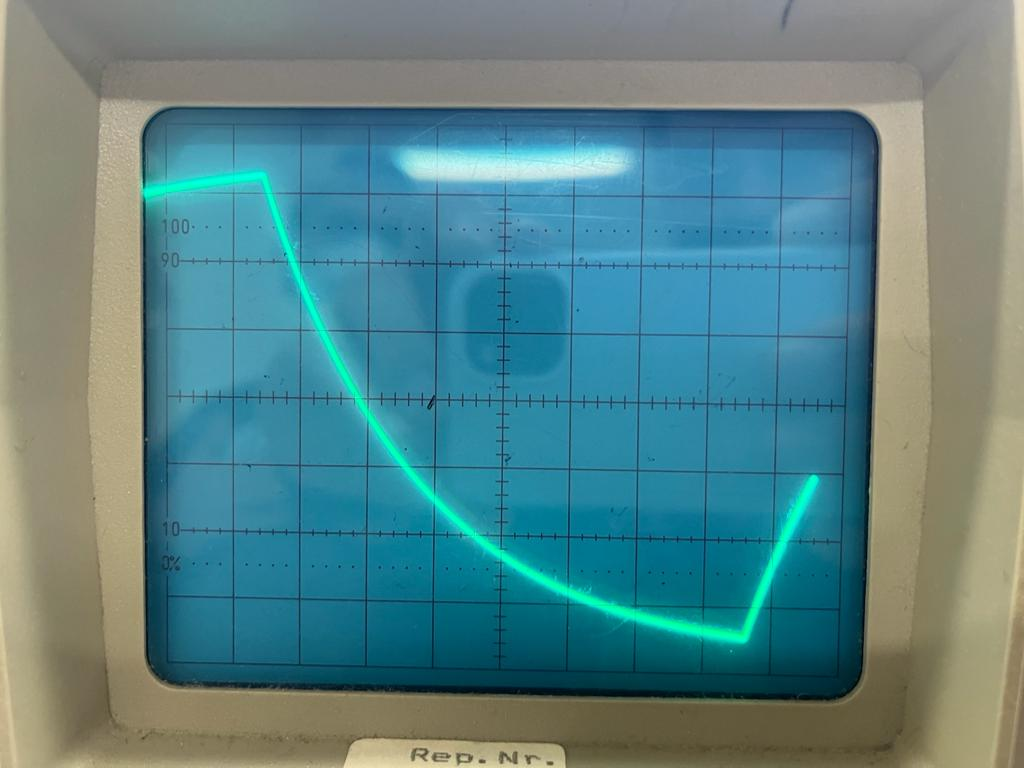
\includegraphics[height=70mm]{bilder/1.jpeg}
    \caption{Entladevorgang des RC-Gliedes bei angelegter Rechtecksspannung.\label{Abbildung3} }
\end{figure}

\begin{flushleft}
    Aus der Aufnahme wurden zehn Wertepaare entnommen und tabellarisch aufgelistet.
\end{flushleft}

\begin{table}[H] 
    \centering
    \caption{$U_{\text{C}}(t)$ zu bestimmten t.} 
    \label{Tabelle1}
    \begin{tabular} {c  c  c }
        \toprule
        {$ U_{\text{C}}(t) \mathbin{/} \unit{\volt} $} &
        {$ ln \left(\frac{U_{\text{C}}}{1\,\unit{\volt}}\right) $} &
        {$ t \mathbin{/} \unit{\milli\second} $} \\
        \midrule
        0,56  & -0,579 & 0,5 \\
        0,44  & -0,820 & 1   \\
        0,28  & -1,272 & 2   \\
        0,175 & -1,742 & 3   \\
        0,14  & -1,966 & 3,5 \\
        0,1   & -2,302 & 4   \\
        0,06  & -2,813 & 5   \\
        0,04  & -3,210 & 5,5 \\
        0,03  & -3,500 & 6   \\
        0,019 & -3,963 & 6,5 \\
        \bottomrule
    \end{tabular} 
\end{table} 

\begin{align}
    \intertext{Für die Zeitkonstante $RC$ lässt sich eine Ausgleichsrechnung mit der Formel (\ref{7}) bestimmen.}
    \ln \left(\frac{U_{\text{C}}}{1\,\unit{\volt}}\right) = m \cdot x + b \label{8}
\end{align}

\begin{figure}[H]    
    \centering
    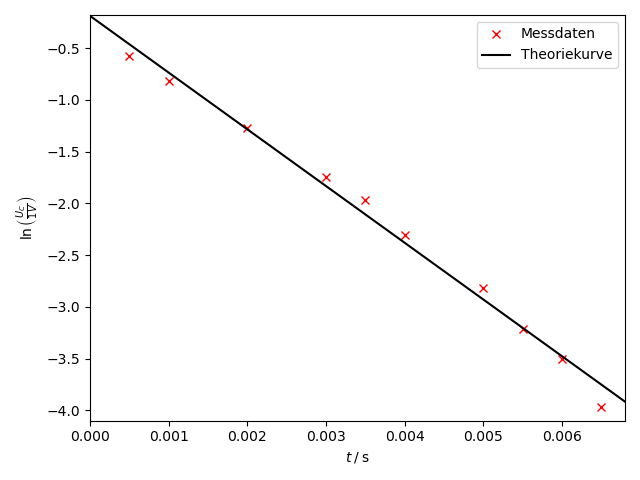
\includegraphics[height=80mm]{bilder/Entladevorgang.png}
    \caption{Bestimmung der Zeitkonstante durch lineare Regression.\label{Abbildung4} }
\end{figure}

\begin{align*}
    \intertext{Die Ausgleichsgerade liefert die Parameter}
    m = (1807,01 \pm 30,50)\,\unit{\second}^{-1} \\
    b = (-0,305 \pm 0,155).
    \intertext{Somit lautet die Zeitkonstante}
    RC_{1} = -\frac{1}{m} = (-5,53 \pm 0,301) \cdot 10^{-4}\,\unit{\second}
\end{align*}

\subsection{Amplitude der Kondensatorspannung in Abhängigkeit von der Frequenz und die Phasenverschiebung}

\begin{flushleft}
    In diesem Teil wird die Kondensatorspannung $U_{\text{C}}$ und die Speisespannung $U_{\text{0}}$ in Abhängigkeit von der Frequenz gemessen.
    Dabei wurden die Amplituden im Bereich von $20\,\unit{\hertz}$ bis $20\,\unit{\kilo\hertz}$ ermittelt. 
    Zudem sind die jeweiligen Abstände $a$ und die Wellenlänge in Bogenmaß $b$ zu finden. 
    Daraus resultiert die Phasenverschiebung $\varphi$.
\end{flushleft}

\begin{table} [H]
    \centering
    \caption{Die Kondensatorspannungsamplitude sowie die Messwerte a und b in Abhängigkeit der Frequenz.} 
    \label{Tabelle2}
    \begin{tabular} {c  c  c  c  c  c  c  c }
        \toprule
        {$ f \mathbin{/} \unit{\hertz} $} &
        {$ U_{\text{C}} \mathbin{/} \unit{\volt} $} &
        {$ U_{\text{0}} \mathbin{/} \unit{\volt} $} &
        {$ \frac{U_{\text{C}}}{U_{0}} $} &
        {$ a \mathbin{/} \unit{\second} $} &
        {$ b \mathbin{/} \unit{\second} $} &
        {$ \varphi \mathbin{/} \text{rad} $} \\
        \midrule
        20    & 0,90  & 0,6 & 1,50   & 0,0010   & 0,05    & 0,12566 \\
        80    & 0,85  & 0,6 & 1,416  & 0,00050  & 0,0125  & 0,25132 \\
        140   & 0,75  & 0,6 & 1,25   & 0,00050  & 0,00714 & 0,43999 \\
        200   & 0,67  & 0,6 & 1,116  & 0,00060  & 0,005   & 0,75398 \\
        600   & 0,35  & 0,6 & 0,583  & 0,00030  & 0,0016  & 1,17809 \\
        1000  & 0,20  & 0,6 & 0,30   & 0,00022  & 0,001   & 1,38230 \\
        2000  & 0,12  & 0,6 & 0,20   & 0,00010  & 0,0005  & 1,25663 \\
        9000  & 0,02  & 0,6 & 0,03   & 0,000026 & 0,0001  & 1,63362 \\
        15000 & 0,013 & 0,6 & 0,0216 & 0,000016 & 0,00006 & 1,67550 \\
        20000 & 0,10  & 0,6 & 0,016  & 0,000012 & 0,00005 & 1,50796 \\
        \bottomrule
    \end{tabular} 
\end{table}

\begin{align*}
    \intertext{Die Ausgleichsfunktion hat die Form}
    \frac{U_{\text{C}}}{U_{0}} = \frac{1}{\sqrt{1+a^2 \cdot f^2}} \\
    \iff \frac{U_{\text{C}}}{U_{0}} = \frac{b}{\sqrt{1+a^2 \cdot f^2}}
    \intertext{Die Funktion wurde mit einem weiteren Regressionsparameter $b$ ergänzt, da einige Werte von $\frac{U_{\text{C}}}{U_{0}} > 1$ sind. }
\end{align*}

\begin{figure}[H]       
    \centering
    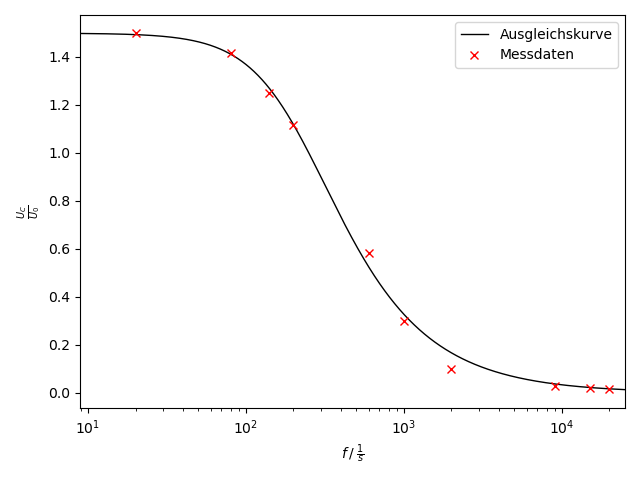
\includegraphics[height=80mm]{bilder/Amplituden.png}
    \caption{Die Abbildung des Frequenzabhängigen Amplitudenverhältnis.\label{Abbildung5} }
\end{figure}


\begin{align*}
    \intertext{Durch die Augleichsrechnung ergibt sich}
    RC_{2} = (4,466 \pm 0,244 )\cdot 10^{-3}\,\unit{\second}.
\end{align*}

\begin{flushleft}
    Die Phasenverschiebung einer externen Sinusspannung und Kondensatorspannung wird in Abhängigkeit von der Frequenz untersucht.
    Zur Bestimmung der Phasenverschiebung wird die Gleichung (\ref{6}) verwendet. 
    Die Messwerte dazu befinden sich in Tabelle \ref{Tabelle2}.
    Dabei wird $\varphi$ gegen die Frequenz geplottet, wodurch sich dann $RC$ bestimmen lässt.
    Zudem wird ein Polarplot erstellt.
\end{flushleft}

\begin{figure}[H]    
    \centering
    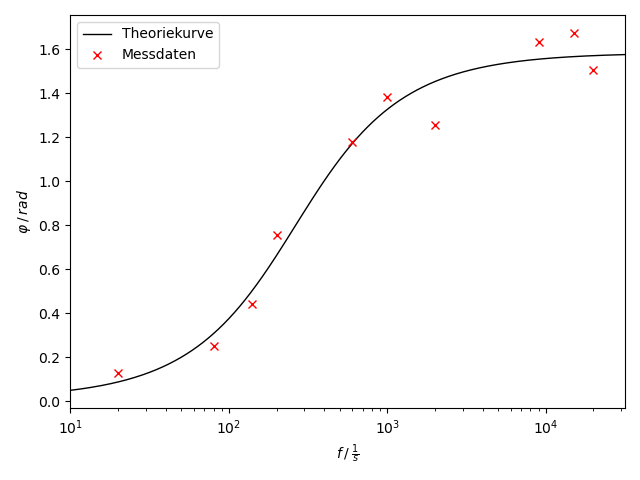
\includegraphics[height=80mm]{bilder/Phasenverschiebung.png}
    \caption{Die Abbildung der Phasenverschiebung.\label{Abbildung6} }
\end{figure}

\begin{align*}
    \intertext{Daraus folgt}
    RC_{3} = ( -1,002 \pm 0,0719 )\cdot 10^{-3}\,\unit{\second}.
\end{align*}

\begin{figure}[H]
    \begin{subfigure}{0.60\textwidth}
        \centering
        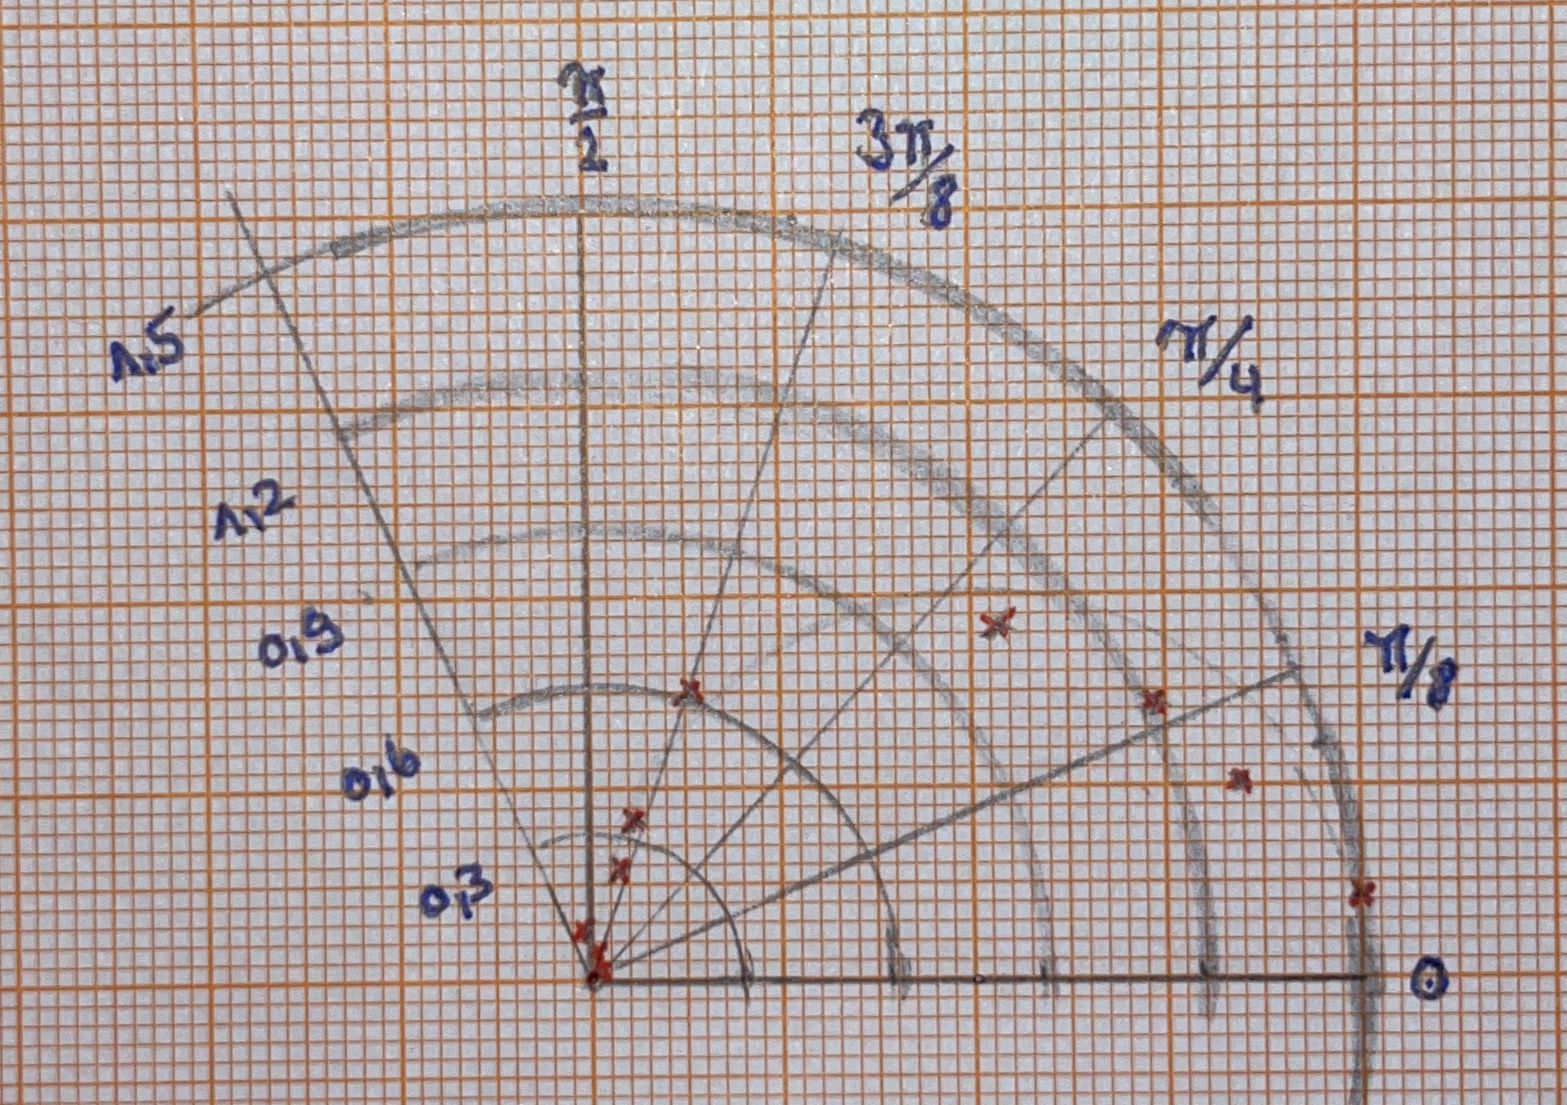
\includegraphics[width=85mm]{bilder/polarbild.jpeg}
        \caption{} 
        \label{}
    \end{subfigure}
    \hfill
    \begin{subfigure}{0.60\textwidth}
        \centering
        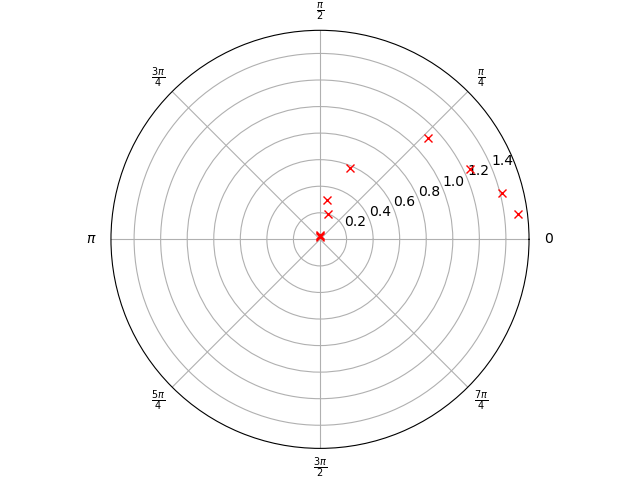
\includegraphics[height=73mm]{bilder/Polarplot1.png}
        \caption{} 
        \label{}
    \end{subfigure}
    \caption{Darstellung der Phasenverschiebung einem Polarplot}
    \label{}
\end{figure}

\subsection{RC-Kreis als Integrator}

\begin{flushleft}
    Im Folgenden wird zur Untersuchung der Integrator-Identität des RC-Kreises drei verschiedene Wechselspannungen angelegt.
\end{flushleft}

\begin{figure}      
    \begin{subfigure}{0.60\textwidth}
        \centering
        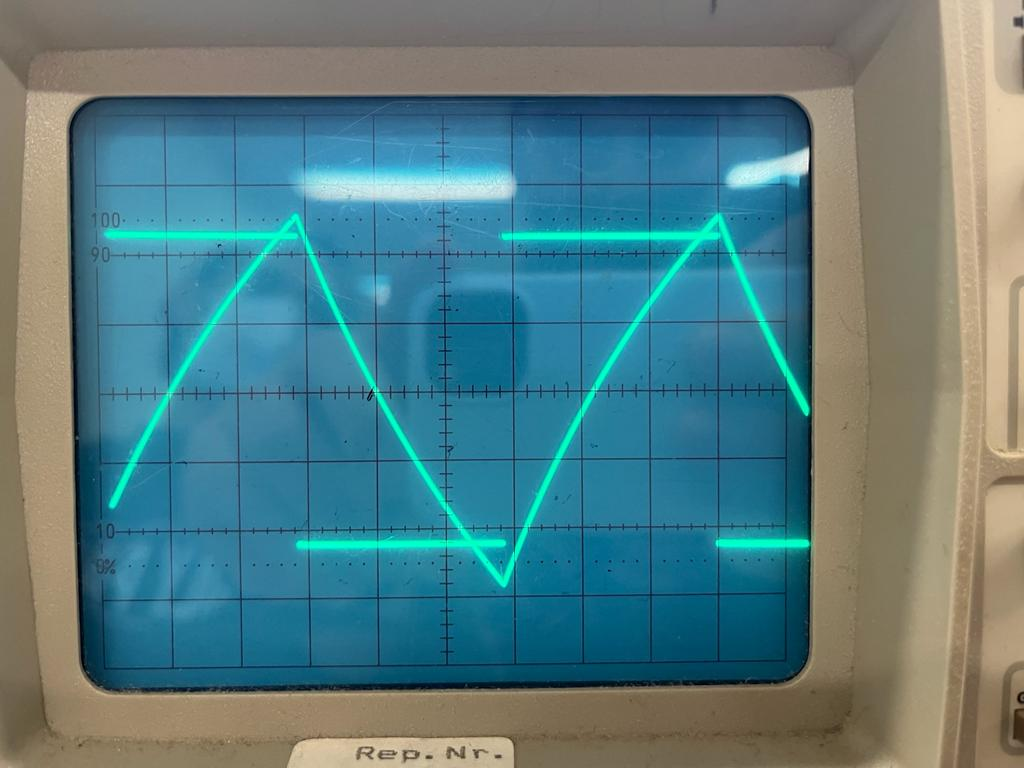
\includegraphics[height=34mm]{bilder/3.jpeg}
        \caption{Die Abbildung der Rechtecksschwingung} 
        \label{Abbildung7a}
    \end{subfigure}
    \hfill
    \begin{subfigure}{0.60\textwidth}
        \centering
        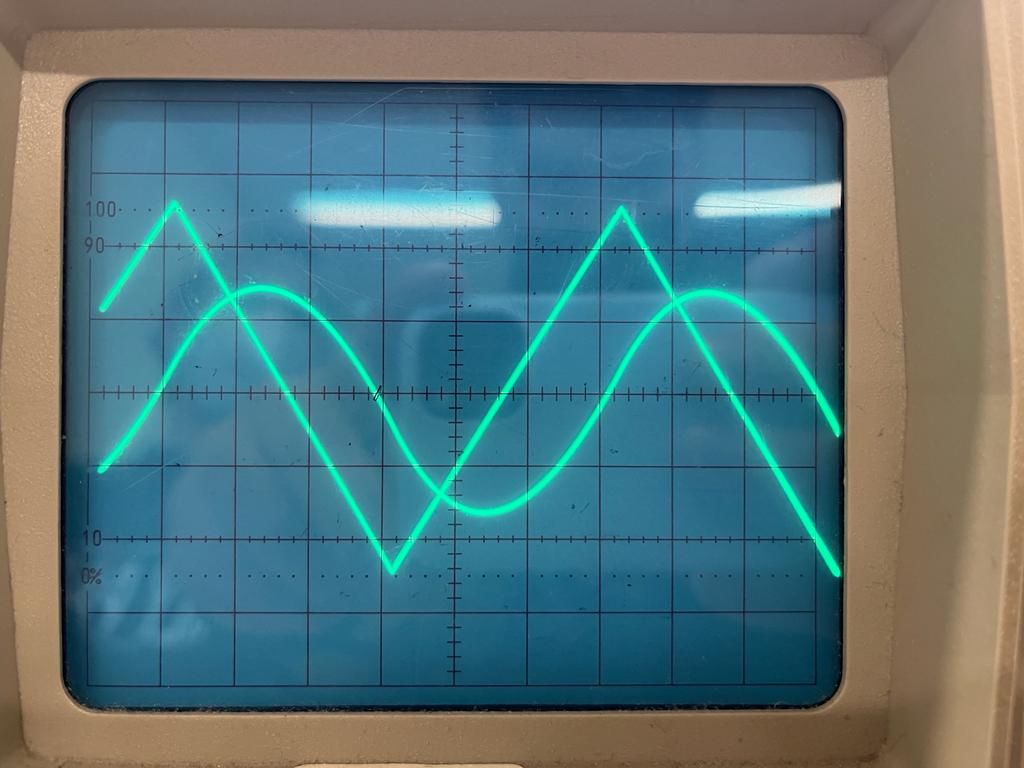
\includegraphics[height=32mm]{bilder/4.jpeg}
        \caption{Die Abbildung der Dreiecksschwingung} 
        \label{Abbildung7b}
    \end{subfigure}
    \center
    \begin{subfigure}{0.60\textwidth}
        \centering
        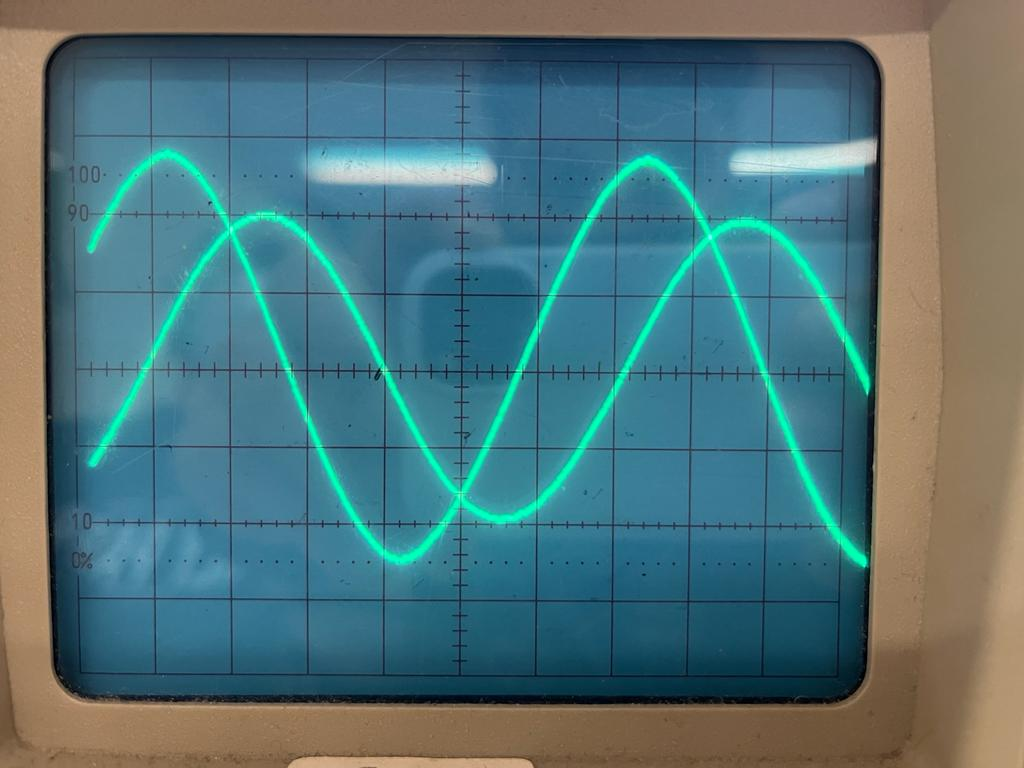
\includegraphics[height=30mm]{bilder/2.jpeg}
        \caption{Die Abbildung der Sinusschwingung} 
        \label{Abbildung7c}
    \end{subfigure}
    \caption{Die drei verschiedenen Wechselspannungen}
    \label{Abbildung7}
\end{figure}
